% g-2 Introduction
\chapter {Introduction} \label{ch:intro}

In particle physics, \gmtwo of the muon, and \gmtwo in general, is an important and deep probe into \tsm (SM). In order to properly introduce the concept of \gmtwo, it is important to first discuss some background fundamentals.  After covering the basics, an argument as to the benefits of measuring \mugmtwo solidifies the scientific context. Then, a brief history of \mugmtwo experiments establishes the context for current \mugmtwo experiments and highlight the gradual rise of statistical tension between measured and calculated results.  And, finally, the state of theory illuminates the types of contributions that affect \mugmtwo and models may resolve the experimental results. 

\section{Magnetic Moments}

\subsection{Definition}
A thorough understanding of \gmtwo begins with classical model for a magnetic moment.  An entity attains a magnetic moment, $\vec{\mu}$, when the object has a certain correlation between the motion of electric charges which it possesses and the physical space it occupies.  Equation \ref{eqn:magnetic-moment-integral} shows the way to calculate such a correlation in a single continuous body or particle \cite{jackson}.  The macro-scale quantity uses the term spin polarization or magnetization, $\vec{M}$, defined in equation \ref{eqn:polarization-sum}.

\begin{equation}
\label{eqn:magnetic-moment-integral}
\vec{\mu} = \frac{1}{2} \int \vec{r} \times \vec{j} \,dV
\end{equation}

\begin{equation}
\label{eqn:polarization-sum}
\vec{M} = \sum_i \vec{\mu}_i
\end{equation}

\noindent
Equation \ref{eqn:magnetic-moment-integral} can be reframed in terms of angular momentum, $\vec{l}$, and charge density, $
\rho$, by noting that $\vec{j} = \rho v$ and $\vec{l} = \vec{r} \times \vec{p}$.

\begin{equation}
\label{eqn:magnetic-moment-integral-2}
\vec{\mu} = \frac{1}{2 m} \int \rho \cdot \vec{l} \,dV
\end{equation}

The angular momentum $\vec{l}$ can be orbital, $\vec{L}$, or intrinsic spin, $\vec{S}$, so the equation holds, classically at least, for volumes and point-like particles with spin. The caveat is that there is a proportionality constant, the g-factor, which must be included in the spin calculation of the equation giving rise to equation \ref{eqn:spin-magnetic-moment} for particle magnetic moments that arise due to spin.

\begin{equation}
\label{eqn:spin-magnetic-moment}
\vec{\mu} = g \frac{e}{2m}\vec{S}
\end{equation}

\noindent
The g-factor, $g$, represents the coupling strength of a particle to the type of interactions mediated by magnetic fields.  This quantity can vary extensively between different particles for instance, the proton g-factor is 5.5, and the neutron has a g-factor of -3.8\cite{codata}.  It is worth noting that naively the neutron should not even have a magnetic moment due to a lack of net charge.  For point-like particles, Dirac calculated the g-factor to be exactly 2 using the relativistic Dirac Equation.  Discrepancies in measurement did not arise for several years, a discussion contained in \ref{sec:history-expt} rather than here.  The overall effect is a shift in the value of $g$ at the \SI{0.1}{\percent} level.

\subsection{Equilibrium}
Intuitively, a magnetic moment is similar to a macro-scale magnet that all children are familiar with.  One prominent behavior exhibited by magnets is a tendency to align with external magnetic fields.  The magnet aligns to minimize potential energy in the external field as given by equation \ref{eqn:spin-b-field-potential}.

\begin{equation}
\label{eqn:spin-b-field-potential}
U = -\vec{\mu} \cdot \vec{B}
\end{equation}

\begin{equation}
\label{eqn:spin-b-field-force}
\vec{F} = \nabla (\vec{\mu} \cdot \vec{B})
\end{equation}

\noindent 
Such macro behavior is used by compasses to align with the Earth's magnetic North Pole and seen with bar magnets where oppositive ends attract.  The behavior persists in the micro as well, and this behavior turns out to be convienient in attaining magnetization for pulsed nuclear magnetic resonance (pNMR) measurements.

\subsection{Precession}
Precession is another prominent and very important behavior arising from the same force on a non-zero magnetic moment in an external magnetic field.  A more familiar analogue comes from the spinning top example.  The child's toy recieves a torque when the normal force between the top's tip and the ground is misaligned with the center of mass. 

\begin{equation}
\label{eqn:top-torque-equation}
\vec{\tau} = \vec{r} \times \vec{F}_{N}
\end{equation}

\begin{figure}
\label{fig:spinning-top-precession}
\centering
\includegraphics[width=0.5\linewidth]{fig/spinning-top-precession}
\caption{The spinning top example of precession as a force diagram.  A torque arises from the off-center normal force, and that torque causes the top to precess at $\omega_p$.  \todo{cite wikipedia source}}
\end{figure}

\noindent
While the top is stabilized by rotational inertia, the induced torque cause the body to rotate about the top's tip.  The magnetic moment case can be realized by allowing the normal force to be replaced by the Lorentz force from the external magnetic field on the effective currents in object with non-zero magnetic moment, equation \ref{eqn:mu-torque-equation}.

\begin{equation}
\label{eqn:mu-torque-equation}
\vec{\tau} = \vec{\mu} \times \vec{B}
\end{equation}

\noindent
The induced torque causes the magnetic moment vector to rotate in plane orthogonal as prescribed by equation \ref{eqn:larmor-precession}. The behavior is referred to as Larmor precession.

\begin{equation}
\label{eqn:larmor-precession}
\omega = \frac{\mu B}{2 m}
\end{equation}

\subsection{Anomaly}
The quantity \gmtwo is realized by taking the g-factor and subtracting Dirac's prediction that the g-factor for a point-like particle should be exactly 2.  Dirac's prediction does not account for any quantum field theory type interactions.  The resulting \gmtwo quantity, equation \ref{eqn:a-lepton} represents only the deviation from the classical value, the anomalous magnetic moment.

\begin{equation}
\label{eqn:a-lepton}
a_{\ell} \equiv \Big(\frac{g\hbox{--}2}{2} \Big)_\ell
\end{equation}

\noindent
Note that the two labels, $a$ and \gmtwo, are used somewhat interchangeably to denote the anomalous magnetic moment even though they technically differ by a factor of two.

\section{Muon Characteristics}

\subsection{Decay Chain}

The pion decay chain is commonly used in the production of spin polarized muons.  The pion and muon decay formulas are given in equation \ref{eqn:pion-decay-chain}.  The principle branching from pion decay produces muons with very high probability, more than \SI{99.9}{\percent} \cite{pdg-2016}.  Similarly, the muon decays into an electron and two neutrinos with nearly \SI{100}{\percent} probability.  The decay formulas are shown in equation \ref{eqn:pion-decay-chain}.

\begin{align}
\label{eqn:pion-decay-chain}
\pi^+ & \rightarrow \mu^+ \bar{\nu}_\mu  & \pi^- & \rightarrow \mu^- \nu_\mu \\
\mu^+ & \rightarrow e^+ \bar{\nu_e} \nu_\mu  & \mu^- & \rightarrow e^- \nu_e \bar{\nu}_\mu 
\end{align}

\subsubsection{Pion Decay}

The two-body decay is isotropic in the pion rest frame and imparts half of the pion mass to both the muon and (anti-)neutrino produced.  In the SM, neutrinos are always produced with left-handed chirality meaning that the direction of the spin direction and the momentum direction are anti-aligned.  Conservation of angular momentum then forces the muon produced via pion decay to have the same chirality as the neutrino.  The decay lends itself to production of a spin polarized muon beam.  When the isotropic decay is boosted into the lab frame for a pion beam, both the highest energy or lowest muons exhibit strong spin polarization, so momentum selection can be used to achieve a polarized muon beam. 

\subsubsection{Muon Decay}

The muon decay is a bit more complicated than pion decay.  The process is a three body decay.  A common framing when talking about muon decay uses a probability distribution and asymmetry function over the range of possible muon energies.  The asymmetry function is a proxy for the likelihood of the decay electron momentum to be in the direction of the muon spin.  It is instructive to examine the extreme cases where both neutrinos are emitted in the same direction and the case where they have opposing momentum directions.  

The first case is the highest energy decay electron, the two neutrinos receive half the decay energy and the electron receieves the other half.  The neutrino/anti-neutrino pair carry away no angular momentum, because the neutrino must have left-handed chirality and the anti-neutrino must have right-handed chirality, opposing spins.  The decay electron then must carry the spin of the parent muon.

The second case is the lowest energy decay electron, the neutrino and the anti-neutrino each receive half the rest mass of the muon.  The electron is produced nearly at rest in that case.  The angular momentum carried by the neutrinos in this case is no longer zero, but rather one.  The electron then will be produced with spin in the opposite direction as the parent muon.

\begin{align}
\label{eqn:muon-decay-distributions}
n_{rest}(y) & = y^2(3 - 2 y) & a_{rest}(y) & = \frac{2 y - 1}{3 - 2y} \\
n_{lab}(y) & = \frac{-8 y^2 + y + 1}{4 y^2 - 5y - 5} & a_{lab}(y) & = \tfrac{1}{5}(y - 1) (4 y^2 - 5y - 5)
\end{align}

\begin{figure}
\label{fig:muon-decay-distributions}
\centering
\includegraphics[width=1.0\linewidth]{fig/muon-decay-distributions}
\caption{Characteristics of the muon decay.  Each plot shows the decay probably as a function of fractional energy, and the decay asymmetry which is a proxy for the probability that the electron emission occurs in the direction of the muon spin.  The left plot shows the distributions for the rest frame of the muon, and the right plot shows the same for the lab frame after boosting to \pmagic.}
\end{figure}

\section{Motivation}
There are two major questions that need answers to specifically motivate the muon \gmtwo experiment.  The first question is: ``Why measure the anomalous magnetic moment?'', and the second question is: ``Why use muons?''.

\subsubsection{Why \gmtwo?}
To the first charge, there are many appropriate replies.  One answer is that it is a simple measurement in principle.  The experimenters need a spin polarized volume of particles, an external vertical magnetic field, and a technique to determine the spin direction. Another, more phenomenological answer is that contributions to \gmtwo come from the full gamut of fundamental interactions and constants of the universe in the SM: Quantum Electrodynamics (QED), Electro-Weak Interactions (EW), and Quantum Chromodynamics (QCD) all playing important roles. It traverses the entirety of Standard Model interactions excepting gravity. Precision measurements of \gmtwo are somewhat unique in this regard, and perhaps for that reason, experimentalists have been fascinated by \gmtwo for many years.

\subsubsection{Why muons?}
And, to the second question, there are physics considerations and practical considerations.  The physics consideration weighs in with the desire for sensitivity to the intricacies of the Standard Model.  Many higher order interactions come into the playing field with mass suppression terms, $\propto (\frac{m_\ell}{M})^2$, or possibly an even higher power.  These terms mostly manifest in the EW and QCD sector.  The relative mass ratio between the electron and the muon enhance these terms by a factor of $(\frac{105.66}{0.511})^2 \approx 43,000$ \cite{the-muon-g-2}!  To that end, the electron \gmtwo is a deeper probe of QED and the muon \gmtwo is a more rounded probe of the SM.  The preceding argument begs the question though: ``Why not use the $\tau$?''.  The answer is really a practical consideration; the ephemeral $\tau$ has a lifetime of only \SI{0.29}{\femto\second} compared to \SI{2.2}{\micro\second} for $\mu$\cite{codata}.  While the $\tau$ particle is appealing if a significant enough Lorentz boost could be achieved, an experiment using $\tau$ particles is simply not practical with current technology.

\subsubsection{Discrepancy}

The muon \gmtwo has been measured many times over the years, and throughout it has remained an interesting probe of the Standard Model.  The experiments are discussed further in section \ref{sec:history-expt}.  Theoretical calculations are similarly discussed more in section \ref{sec:theory}.  The precision of measured and calculated \mugmtwo values have kept similar pace over the year, no doubt due to pushes on one front inspiring pushes on the other, and the progression of the value can be seen in figure \ref{fig:intro-historical-values}.  The path of theory and experiment split over the years to arrive at the current values which exhibit a \SI{3}{\sigma} statistical tension.  The persistent statistical tension is viewed as a possible indication of new physics from beyond \tsm.

\begin{figure}
\label{fig:intro-historical-values}
\centering
\includegraphics[width=0.9\linewidth]{fig/intro-historical-values}
\caption{The progression of theoretical and experimental values for \mugmtwo over the years.  A clear divergence in each can be seen as the precision for each increases.  The latest inputs place the statistical tension between theory and experiment at about \SI{3}{\sigma}. Note that all points are drawn with uncertainty bars, but the markers themselves are larger than the uncertainty on some points. \todo{add theory values, add uncertainty bands}}
\end{figure}

\subsubsection{Implementations}

What then, one might ask, are the bare necessitites to perform the \gmtwo experiment?  Number one is reliable source of spin polarized muon, the higher the net polarization the better.  Next, the there must be a method to store the muons in an external magnetic field while they precess which can be achieved through a penning trap setup as in older experiments or a cyclotron storage ring as in many newer experiments.  The third necessesity is is a method by which to measure the direction of the muon spin vector over time.  Measuring the spin direction relies on on the fact that spin informations is transfered to the momentum of the decay electron.  The detector could be as simple as a forward/backward electron sensitive detector that catches decay electrons.  The last requirement is a measuremenent of the magnetic field experienced by the muons as they precess.  Keep these issues in mind as the historical experiments are discussed in the following sections.

\section{History of Experiment} \label{sec:history-expt}

\subsection{Anomaly Detection and Parity Violation}

The notion that $g \ne 2$ had to be reconciled with experiment as measurement precision progressed and statistical tensions arose with the values predicted by theory.  Deviations from a pure Dirac particle for leptons were first observed in hyperfine splitting measurements of several different isotopes by Kusch and Foley in 1947 \cite{kusch-foley}.  The theory community quickly resolved the discrepancy when Julian Schwinger released his seminal paper introducing corrections from quantum field fluctuations in 1948 \cite{schwinger}.  The paper describes a now standard QED calculation of the lowest order self-interaction for leptons emitting and reabsorbing photons, see figure \ref{fig:schwinger-diagram}.  The Schwinger term brought experiment and theory back into good agreement, an early triumph of QED.

\begin{figure}
\label{fig:schwinger-diagram}
\centering
\includegraphics[height=\fdh]{fig/schwinger-diagram}
\caption{The Feynman diagram for the so-called Schwinger term. The propogating lepton radiates a photon, interacts with the magnetic field via a disconnected photon and re-absorbes the radiated photon.  The contribution to $a_\mu$ from the interaction is $\frac{\alpha}{2\pi}$.}
\end{figure}

The first detection of a magnetic moment anomaly from measurements of free electrons came later, and in muons much later.  The first measurement of $g_e$ happened in 1953 by H. R. Crane, et al. \todo{can't find pdf of paper}.  Subsequent theoretical calculations and supporting experimental measurements established $g_e$ as the most precisely predicted and measured quantity of QED.  \todo{Add reference for $g_e$ review}.  As for measuring $g_\mu$, it wasn't clear how to properly control the polarization of the muons, that is until parity violation of the Weak interaction came to light.  With parity violation baked into the Weak interactions, researchers quickly realized that a pion beam would decay into muons polarized along the beam direction (see section \ref{sec:muon-production} for more detail on pion decay).

\subsection{CERN-I}
Building off the Weak parity revelation, researchers measured $g_\mu$ for the first time.  In 1960 Columbia personnel measured the quantity to $5\%$ uncertainty, and not long after a more precise measurement came out of CERN and eclipsed it.  The experiment worked by injecting relatively low energy, \SI{83}{\MeV}, muons into a long, narrow magnetic trap where the polarized muons would undergo both cyclotron motion and lateral drift, see figure \ref{fig:cern-i-diagram}. At the opposite end of the magnet, the muons were ejected, tagged for storage time, and stopped where the momentum direction of the decay electron was recorded as either forward or backward.  Using this technique CERN scientists were able to achieve a precision of $0.4\%$, absolutely phenomenal for the time\cite{cern-i}.  At the achieved precision, a deviation of $1.6\,\sigma$ was present between the measured value and the value predicted using the Schwinger term\cite{47y-muon-g-2}.

\begin{figure}
\centering
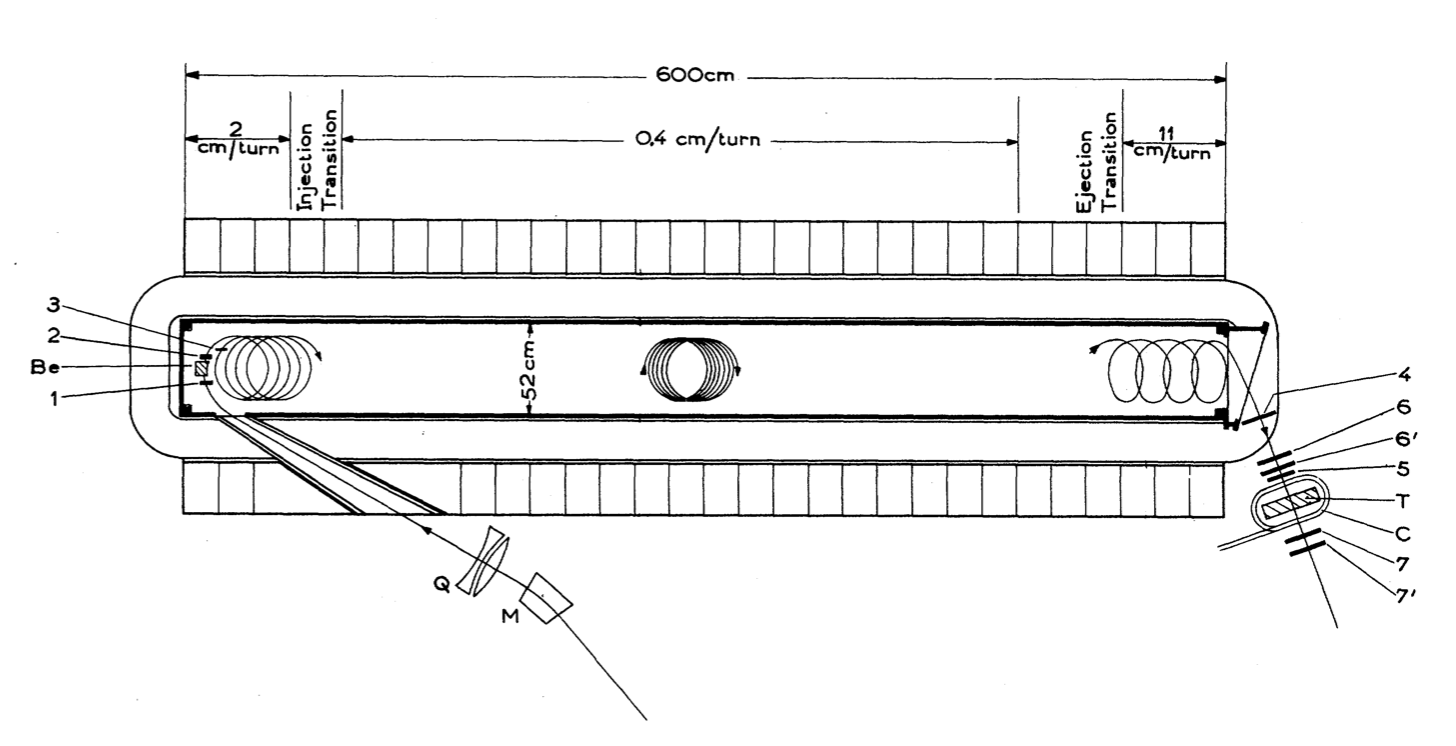
\includegraphics[width=0.9\linewidth]{fig/cern-i-diagram.png}
\label{fig:cern-i-diagram}
\caption{A diagram of the experimental setup in the first muon \gmtwo experiment at CERN from the original paper\cite{cern-i}. The muons enter from the lower left, go through the energy moderator to put the cyclotron radius at 19cm, drift and circles toward the ejection side of the magnetic, escape from the the magnet, stop in the fiducial block, and decay into an electron with momentum correlated to the spin direction.}
\end{figure}

\subsection{CERN-II}
The second iteration of \mugmtwo at CERN improved by a factor of 15 over the first!  CERN-II was the first \mugmtwo to use the now familiar storage ring.  The storage ring design allowed the experimenters to measure \gmtwo directly as opposed to $g$ as explained in section \ref{sec:expt-big-picture}. In order to store muons, the experiment injected a beam of protons which hit a pion production target.  A slice of the pion production phase space matched the momentum acceptance of the ring well enough to remain for several revolutions. And, some fraction of the muons produced from pion decay were mostly forward decays that lost a bit of energy and matched the ring's momentum acceptance.  The decay electrons curled inward to electron counting detectors at a rate modulated at \gmtwo frequency.  The injected muons had a relativistic $\gamma$ of 12 which allowed the researchers to increase the observation time of muon spin precession to more than 130 $\mu s$.  The increased duration led to improved determination of $a_\mu$ to \ppm{270}\cite{47y-muon-g-2}.

\subsection{CERN-III}
The final CERN muon \gmtwo experiment ran from 1969 to 1976.  A major innovation introduced in CERN-III was use of the so-called "magic" momentum. Observe equation \ref{eqn:full-omega-a}, the expression for spin precession in electromagnetic fields for a relativistic muon.

\begin{equation}
\label{eqn:full-omega-a}
\omega^\prime_a = \omega_a[1 + (1 - 1 / a \beta^2 \gamma^2)(\beta E_r / B)]
\end{equation}

\noindent A muon beam at a very specific momentum, \pmagic, cancels the effects of radial electric fields which allows electrostatic focusing to be used on the muon beam instead of magnetic gradient focusing.  The perturbations from magnetic focusing was a large source of uncertainty in the previous experiment.  Another major innovation for the third CERN experiment was the use of pion injection instead of proton injection.  The measurement techniques of CERN-III were similar to CERN-II.  With the achieved improvements, the CERN team was able to drive down the uncertainty on $a_\mu$ to \ppm{7}\cite{47y-muon-g-2}, nearly a 40-fold improvement!

\subsection{E821 at BNL}
The most precise \mugmtwo experiment to date, took place at Brookhaven National Laboratory (BNL). The experiment, E821 as it is labeled in high energy physics ledgers, pushed precision muon phyiscs to the next level.  The precision goals for E821 demanded a 400-fold increase in statistics over its predecessor.  In order to accommodate the necessesited higher rates, the decay electron measurement platform was separated into 24 individual calorimeters.  Another critical improvement in the experiment, E821 injected muons rather than pions, or protons.  Muon injection provided a cleaner data earlier in each injection, and with an exponentially decaying number of muons, an early start time could be a huge rate improvement.  The experiment design also focused on improving the homogeneity of the magnetic storage field.  The aperture of the storage region was increased to facilitate a more uniform magnetic field across the muon storage volume.  Field measurement was also improved by implementing both a suite of stationary magnetometers outside of the storage region to continuously monitor magnetic field drift and a trolley outfitted with an array of 17 magnetometers to measure the field in the storage volume periodically.  

In the end, the experiment nearly reached the initial goal of 350 ppb uncertainty on $a_\mu$, actually achieving 540 ppb uncertainty\cite{e821-prd}.  The E821 \gmtwo result was at odds with theoretical calculations.  Depending on which theoretical models were employed, the measurement was somewhere around $3.3\sigma - 3.6\sigma$ away from theoretical prediction, a statistical tension!

\subsection{Contemporary Experiments}
The tension remained in subsequent years, inspiring a new iteration of the \mugmtwo experiment at Fermi National Accelerator Laboratory (FNAL). The experiment, E989, reuses the storage ring, superconducting coils, and various components from the BNL experiment.  The precision goal of E989 is an overall uncertainty of 140 ppb, likely pushing the tension to discovery levels, i.e., \SI{5}{\sigma}. Additionally, a sister experiment is underway at J-PARC as a completely independent measurement of \mugmtwo with similar sensitivity as the BNL experiment.  In a parallel effort, theoretical particle physics researchers have been pushing the precision of calculations to match pace with experiment\cite{e989-tdr}.

\section{Theory Contributions} \label{sec:theory}

The theoretical contributions to \mugmtwo come from all corners of particle physics.  The typical diagonalization of the contributions breaks them into QED, EW, and QCD as layed out in equation \ref{eqn:sm-contributions}. The relative sizes of the contributions are displayed in figure \ref{fig:sm-contributions}. The Electro-Weak contributions are well modeled, and theoretical progress involves calculating increasingly intricate Feynman diagrams.  The Strong contributions are trickier and represent a larger challenge to the theory community.  The theory community has set a similar precision goal as the E989 collaboration, \SI{140}{ppb}, following a similar time frame, around 2020\cite{e989-tdr}.

\begin{equation}
\label{eqn:sm-contributions}
a_\mu = a_{_{QED}} + a_{_{EW}} + a_{_{QCD-HVP}} + a_{_{QCD-HLbL}}
\end{equation}

\begin{figure}
\label{fig:sm-contributions}
\centering
\includegraphics[width=1.0\linewidth]{fig/SM-contributions.pdf}
\caption{The spectrum of theoretical contributions to \mugmtwo compared to the experimental value.  The value from each storage ring experiment is represented as a vertical line with the projected precision for E989 as a solid line.  The size and uncertainty of various SM corrections grouped by interaction type are depected as bars extending onto the vertical axis. The most important point highlighted by the figure is that theory only needs to improve in the hadronic light-by-light and hadronic vacuum polarization sectors.}
\end{figure}

\subsection{QED Effects} \label{s-sec:theory-qed}

The correction from QED interactions is the lionshare of $a_\mu$.  Feynman diagrams provide a convenvient way to intuit some of the relevant effects, and the QED effects can be divided into a few different types of interaction diagrams.  One diagram is of the radiative correction type, shown in figure \ref{fig:qed-feynman-diagrams} (1\hbox{--}4).  These diagrams involve emission and recapture of a photon(s) while the particle is in flight.  Another common type of diagram illustrates vacuum polarization interactions, shown in figure \ref{fig:qed-feynman-diagrams} (5\hbox{--}6), which resemble radiative correction with the offshell photon going through pair production and annihilation along its path.

\begin{figure}
\label{fig:qed-feynman-diagrams}
\centering
\includegraphics[height=2.0\fdh]{fig/qed-feynman-diagrams}
\caption{Several examples of QED interactions illustrated as Feynman diagrams.  The first four constitute radiative corrections, and the last two are termed vacuum polarization effects. \todo{Make cleaner diagrams}}
\end{figure}

The QED corrections constitute over 99\% of the total anomalous magnetic moment and the bulk of that arises from the lowest order term.  A natural way to represent QED corrections is through a power series in the QED coupling constant, $\alpha_{_{QED}}$.

\begin{equation}
\label{eqn:qed-correction-series}
a_{_{QED}} = \sum_n{A_n \left(\frac{\alphaQED}{\pi} \right)^n}
\end{equation}

\noindent
The sole first term in the series is the leptonically universal Schwinger term, $a_{_{Schwinger}} = \frac{\alphaQED}{\pi}$.  In terms of the measured value of \gmtwo of the electron, the Schwinger term is $100.134\%$ of the measured value. And for the muon \gmtwo, the lowest order term is a slightly larger fraction of the total at $99.59\%$ \cite{codata}.  In both cases though, the Schwinger term absolutely dominates the corrections.

\begin{align*}
a_{e}   & = 115\;965\;218.091(26) \times 10^{-11} \\
a_{\mu} & = 116\;592\;080(63) \times 10^{-11} \\
a_{_{Schwinger}} & = 116\;120\;635.555(27) \times 10^{-11}
\end{align*}

For higher order terms in the QED correction, one can garner some intuition by investigating a vertex expression in the different mass limits.  First, consider the case of radiative corrections in which the radiated particles are light compared to the muon, $m_p \ll m$.  Equation \ref{eqn:qed-2nd-order-small-m} is a catch-all expression for 2nd order terms in the small mass limit \cite{the-muon-g-2}.

\begin{equation}
\label{eqn:qed-2nd-order-small-m}
\delta a_\mu^p \sim \big(\frac{\alpha}{\pi} \big)^{n_p} \ln^{k_p}\frac{m}{m_p}
\end{equation}

\noindent
And, now consider the opposite case where $m_p \gg m$.  The expression changes to equation \ref{eqn:qed-2nd-order-large-m}.

\begin{equation}
\label{eqn:qed-2nd-order-large-m}
\delta_\mu^p \sim \big(\frac{\alpha}{\pi} \big)^{n_p} \\
\frac{m_p^2}{m^2} \ln^{k_p}\frac{m}{m_p}
\end{equation}

\noindent
The mass supression term can be understood as a result of the fact that these type of muon interactions with heavier particles requires helicity flips for the muon which add a $\frac{m_\mu}{m_p}$ factor and that vertex in the end is squared to yield an amplitude \cite{amm-of-muon}.

The two equations, \ref{eqn:qed-2nd-order-large-m} and \ref{eqn:qed-2nd-order-small-m}, offer insight into the difference between muon and elecron \gmtwo.  The electron mass is much smaller than the muon, so these are the type of higher order interactions that are enhanced in the muon \gmtwo.  Another insight following from the first is the fact that since the electron effects are heavily suppressed, the electron \gmtwo can be used to calculate a very precise value of $\alphaQED$ \cite{amm-of-muon}.

The contribution of QED effects have been calculated out to 5 loops\cite{5-loop-qed}.  That includes more than 10,000 diagrams!  The resulting contribution to \mugmtwo in total is given below.

\begin{equation}
\label{eqn:qed-total}
a_\mu^{^{QED}} = 116\;584\;718.845(0.037) \times 10^{-11}
\end{equation}

\subsection{EW Effects} \label{s-sec:theory-ew}

In general corrections due to the Weak Force are mass suppressed compared to QED corrections, and therefore smaller in stature.  The lowest order and largest contribution to the Weak corrections comes two diagrams, see figure \ref{fig:weak-lowest-order-diagrams}. One is similar to the Schwinger Diagram, the difference being that the photon propagator has been substituted for the Z boson.  The second entails emission of a muon neutrino, conversion to a W boson of the appropriate charge, and recapture of the neutrino.  The expression, eqn. \ref{eqn:weak-lowest-order} for the diagrams is calculated in\cite{the-muon-g-2} where the first term in brackets is derived for the W boson interaction and the second term for the Z boson.  The total contribution for the lowest order Weak corrections is then \SI{194.9}{\times 10^{-11}}.

\begin{figure}
\label{fig:weak-lowest-order-diagrams}
\centering
\includegraphics[height=\fdh]{fig/weak-lowest-order-diagrams}
\caption{The largest contributing diagrams from the Weak Interaction.  The muon in the left diagram goes off shell by emitting and re-absorbing a neutral Z or Higgs boson.  And, the muon in the right diagram converts to a $W^{-}$ ($W^{+}$ for $\mu^{+}$) and emits and re-absorbs a muon neutrino to conserve fermion number.}
\end{figure}

\begin{equation}
\label{eqn:weak-lowest-order}
a_\mu^{weak} = \frac{G_F m^2}{8\sqrt{2}\pi^2} \\
\left[\frac{10}{3} + \frac{1}{3} \left(-5 + (1 - 4\sin{\theta_W}^2)^2 \right) \right]
\end{equation}

The next order in EW interactions might be expected to be nearly negligible.  Naively, they would be suppressed by a coupling factor of $\frac{\alpha}{\pi} \approx 0.002$, and so would amount to a small effect.  However, the contribution also gets an enhancement due to the large logarithm of $\log(m_Z/m) \approx 6.8$, and conincidentally many terms add coherently.  More difficulty arises as QCD effects arise within the Weak boson propagators.  An effect that will not receive more than a mention here.  The total contribution from the second order Weak diagrams ends up being \SI{-40}{\times 10^{-11}}\cite{the-muon-g-2}.  The total contribution to $a_\mu$ is given in equation \ref{eqn:ew-total}. 

\begin{equation}
\label{eqn:ew-total}
a_\mu^{^{QED}} = 154(2) \times 10^{-11}
\end{equation}

\subsection{QCD Effects} \label{s-sec:theory-qcd}

The QCD sector is undoubtedly the most difficult domain to calculate accurately and precisely in determining \gmtwo of the muon.  In general QCD calculationas can be extremely difficult owing to the non-perturbative nature of many QCD problems, and \mugmtwo calculations are no exception.  Some calculations leverage effective low-energy perturbation theories, others chiral perturbation approaches, and others still utilize lattice calulations\cite{the-muon-g-2}.  The comprehensive approach involves both model-dependent calculations and model-independent contributions.  Sorting the bevy of contributions is a daunting task, fortunately muon \gmtwo theory reviews have already done just that for experimentalists.

\subsubsection{Hadronic Vacuum Polarization}

The general form of hadronic vacuum polarization is quite similar to the QED vacuum polarization described in section \ref{s-sec:theory-qed}.  The muon radiates an photon or emits another boson, and the newly created particle pair produces then annihilates before recapture with the muon, illustrated in figure \ref{fig:qcd-hvp-feynman-diagram}.  The difference being that in this case the pair production pulls from the hadronic sector instead of the lepton sector.  Such possibilities include: $\pi_0$, $\pi^+\pi^-$, $\rho_0$, etc.  The size of the HVP correction is second only to the QED correction coming in at around \SI{6000}{\times 10^{-11}}.  

\begin{figure}
\label{fig:qcd-hvp-feynman-diagram}
\centering
\includegraphics[height=\fdh]{fig/qcd-hvp-feynman-diagram}
\caption{The basic diagram for hadronic vacuum polarization.}
\end{figure}

The hadronic vacuum polarization is tricky to anchor to a real world parameter.  The general method employed uses the integral relationship given as

\begin{equation}
\label{eqn:qcd-hvp-integral}
a_\mu^{hvp} = \frac{\alpha}{3\pi} \int_{s_0}^{\infty} \frac{ds}{s} \\
\frac{\sigma_{hadr}(s)}{\sigma_{point}(s)} a_\mu^{(1)}(s)
\end{equation}

\noindent
where $a_\mu^{(1)}(s)$ is the 1-loop contribution to $a_\mu$ from a neutral vector boson with mass $\sqrt{s}$, $\sigma_{hadr}$ is the $e^+e^-$ hadronic annihiliation cross-section, and $\sigma_{point}$ and further detail is given reference\cite{amm-of-muon}.  With the data-driven method employed it is technically possible to get the value exactly.  The reality of the calculation turns out to be difficult, since data from many different experiment needs to be well understood and combines to cover the whole spectrum.  The value could possibly be improved by adding additional cross-section data or through a lattice based approach.  The currently value is given as

\begin{equation}
\label{eqn:qcd-hvp-total}
a_\mu^{^{QCD-HVP}} = 6934(63) \times 10^{-11}.
\end{equation}

\subsubsection{Hadronic Light-by-Light}

The general form for hadronic light-by-light (HLbL) is more intricate than HVP and, as is to be expected, therefore a smaller contribution to the total.  The core idea of hadronic light-by-light scattering is that propagating muon interacts with only three photons and those photons interact with some sort of QCD loop which interacts with the external field.  The HLbL scattering is one of the most difficult $a_\mu$ contributions to calculate, because it cannot be anchored back to experimental data using a dispersion relation like the HVP contribution\cite{the-muon-g-2}.

\begin{figure}
\label{fig:qcd-hlbl-feynman-diagram}
\centering
\includegraphics[height=\fdh]{fig/qcd-hlbl-feynman-diagram}
\caption{The basic diagram for hadronic light-by-light scattering.  The propagating muon interacts with a QCD black box which interacts with the disconnected photon diagram, i.e., the external field.}
\end{figure}

The value is largely model dependent for $a_\mu^{^{HLbL}}$.  The most discussed model in reference\cite{amm-of-muon} uses a color extension allowing a large number of colors and includes constraints from chiral and short-distance QCD.  Other model calculations arrive at values up to 50\% different, but most are closer.  Many groups working in the field convened to establish the Glasgow Consensus as an agreed value for the correction\cite{e989-tdr}.  The consensus value is

\begin{equation}
\label{eqn:qcd-hlbl-total}
a_\mu^{^{QCD-hlbl}} = 105(26) \times 10^{-11}.
\end{equation}

\subsection{Beyond the Standard Model}

\todo{Reframe this in similar terms as Czarnecki and Marciano}

Consider the simplest extensions of the Standard Model where a new particle comes in analagous to a current particle.  A general argument can be made for an approximation of the size of the correction from such diagrams\cite{the-muon-g-2}.  For light particles where the new particle mass is less than the muon mass, $m_p < m_\mu$, the contribution is expected to have the following form:

\begin{equation}
\label{eqn:bsm-general-small-m}
\delta a_\mu \sim \left(\frac{\alpha}{\pi}\right)^{n_p} \left( \ln{\frac{m_\mu}{m_p}} \right)^{k_p}
\end{equation}

\noindent
where the exponent $n_p$ represents the loop order of the correction and the exponent $k_p$ is the possible logarithmic enhancement at the order.  Note that $k_p < n_p$, but not otherwise predictable.

The situation changes a bit when more massive particles are considered, because helicity flips must be accounted for.  In general those helicity flips add a unitless mass suppression term to the vertex function which is squared in the amplitude, so we get the following relation:

\begin{equation}
\label{eqn:bsm-general-large-m}
\delta a_\mu \sim \left(\frac{\alpha}{\pi}\right)^{n_p} \\
\left(\frac{m_\mu}{m_p}\right)^2 \\
\left(\ln{\frac{m_\mu}{m_p}} \right)^{k_p}
\end{equation}

\subsubsection{Supersymmetric Extensions}
With these two general estimates established, it is instructive to talk about a few specific types of corrections.  Supersymmetry(SUSY) is one proposed theory that can account for the deviation in $a_\mu$ with some tuning.  Supersymmetric particles arise through smuon-neutralino and sneutrino-chargino conversions in loop diagrams such as figure \ref{fig:bsm-susy-diagrams}.  A general expression for contributions from SUSY is given in eqn. \ref{eqn:bsm-a-mu-susy}\cite{a-mu-harbinger}.  In equation \ref{eqn:bsm-a-mu-susy}, $\tilde{m}$ is the mass of the SUSY particle

\begin{figure}
\label{fig:bsm-susy-diagrams}
\centering
\includegraphics[height=\fdh]{fig/bsm-susy-diagrams}
\caption{Two example diagrams of SUSY which would contribute to the anamalous magnetic moment. In the left diagram, the muon converts into the supersymmetric particles, the sneutrino, $\tilde{\nu}$ and chargino $\tilde{\chi}$, and back to the muon.  In the right diagram the muon undergoes a different supersymmetric interaction vertex to become a smuon, $\tilde{\mu}$, and a neutralino, $\tilde{\chi}^0$.  These one-loop diagrams are expected to be the largest contributors from minimal SUSY extensions of the SM.}
\end{figure}

\begin{equation}
\label{eqn:bsm-a-mu-susy}
|a_\mu^{SUSY}| \approx \\
\left(\frac{\alpha(M_z)}{8 \pi \sin^2{\theta_W}} \right) \\
\left( \frac{m_\mu}{\tilde{m}} \right)^2 \tan{\beta} \\
\left(1 - \frac{4\alpha}{\pi}\ln{\frac{\tilde{m}}{m_\mu}} \right) \\
\approx 130 \times 10^{-11} \\
\left(\frac{100 GeV}{\tilde{m}} \right)^2 \tan{\beta}
\end{equation}

\subsubsection{Radiative Extensions}
Another proposed theory, radiative mass models can explain both deviations from \gmtwo and the ``unnaturally'' light mass of the leptons.  In this model the mass of the muon is generated by emission and absorption of an as of yet unkown particle while it propagates, and the bare mass of the muon is zero.  The same new particle that provides mass would come in to the anomalous magnetic moment as an unnacounted for Schwinger-like term.  The size of the contributions in such a model are given in eqn. \ref{eqn:bsm-general-small-m}, and the diagrams in figure \ref{fig:bsm-radiative-diagrams}\cite{a-mu-harbinger}.

\begin{figure}
\label{fig:bsm-radiative-diagrams}
\centering
\includegraphics[height=\fdh]{fig/bsm-radiative-mass-diagrams}
\includegraphics[height=\fdh]{fig/bsm-radiative-a-mu-diagrams}
\caption{Example diagrams which would cause the mass of the muon and corrections to \mugmtwo.  The letters represent possible new scalar (S), pseudoscalar (P), and fermion (F) particles.}
\end{figure}

\subsubsection{Other Extensions}

Many other SM extensions have been proposed throughout the years.  See reference \cite{a-mu-harbinger} for a larger list, but a few are listed here.  Dark photons are light, but very weakly coupling particles that could account for \mugmtwo.  Anomalous properties of the W boson, such as anomalous magnetic moment and electric quadrupole, have been proposed as a possible explanation.  Also, new gauge bosons models illustrate a possible avenue for anomalous \gmtwo.

Much of the phase space for the proposed standard model extensions has been impinged upon by other measurements.  The LHC for instance has constrained the parameters in many SUSY models and dark photons.  However, most models are not completely ruled out, and the assay of possible solutions will need to be careful pruned and tuned by the theory community in the coming years.
